\documentclass[11pt, addpoints, answers]{exam}

\usepackage{amsmath, amssymb}
\usepackage{xcolor}

\newcommand{\red}[1]{\textcolor{red}{#1}}

% For inserting code snippets.
\usepackage{listings}
\lstset{
    columns = fixed,
    basewidth = {0.5em},
    breaklines = true,
    backgroundcolor = \color{white},
    keywordstyle = \color[RGB]{40, 40, 255},
    numberstyle = \footnotesize\color{darkgray},
    commentstyle = \ttfamily\color{violet},
    basicstyle = \ttfamily,
    stringstyle = \ttfamily\color[RGB]{128, 0, 0},
    showstringspaces = false,
    language = {[11]C++},
    escapechar = \@
}
\lstnewenvironment{cpp}[1][]{\lstset{language = {[11]C++}, #1}}{}

\usepackage{tikz}
\usepackage{tikz-qtree}
\tikzset{every tree node/.style={minimum width=2em,draw,circle},
    blank/.style={draw=none},
    edge from parent/.style=
    {draw,edge from parent path={(\tikzparentnode) -- (\tikzchildnode)}},
    level distance=1.2cm}

% headers, footers, titles
\newcommand{\CourseName}{CS101 Algorithms and Data Structures}
\newcommand{\HomeworkNO}{Homework 6}
\newcommand{\DueDate}{Due date: November 19, 2023, at 23:59}

\pagestyle{headandfoot}
\runningheadrule
\runningheader{\CourseName}{\HomeworkNO}{\DueDate}
\runningfooter{}{\thepage}{}

\title{
	\CourseName\\
	Fall 2023\\
	\HomeworkNO
}
\author{}
\date{\DueDate}

% formats of questions, choices, points, etc.
\qformat{\bf\thequestion. (\totalpoints\ points) \thequestiontitle\hfill}
\pointname{'}
\CorrectChoiceEmphasis{\bf\color{blue}}
\SolutionEmphasis{\color{blue}}

% We frequently use this font.
\newcommand{\ttt}{\texttt}
\newcommand{\bluett}[1]{\textcolor{blue}{\ttt{#1}}}

\begin{document}

\maketitle

\begin{enumerate}
    \item Please write your solutions in English.
    \item Submit your solutions to gradescope.com.
    \item Set your FULL name to your Chinese name and your STUDENT ID correctly in Account Settings.
    \item If you want to submit a handwritten version, scan it clearly. \ttt{CamScanner} is recommended.
    \item When submitting, match your solutions to the problems correctly.
    \item No late submission will be accepted.
    \item Violations to any of the above may result in zero points.
\end{enumerate}

\begin{questions}

    \newpage

    \include{multiple_choices}

    \newpage

    \titledquestion{AVL tree operations}

Here is an AVL tree. Denote it as $T$.
\begin{center}
    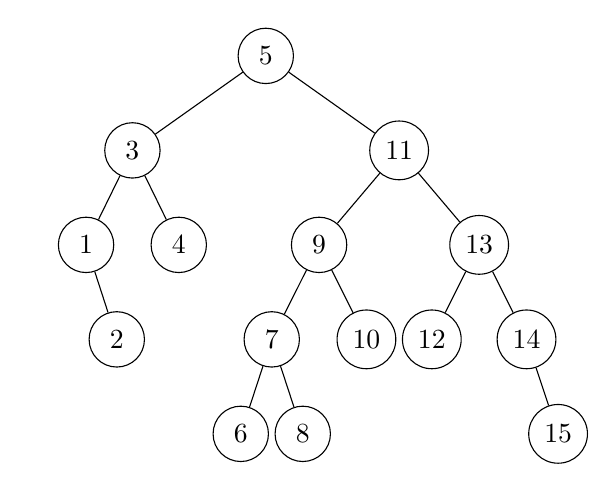
\begin{tikzpicture}[]
        \Tree
        [.5
        [.3
        [.1
        \edge[blank]; \node[blank]{};
        [.2
        ]
        ]
        [.4
        ]
        ]
        [.11
        [.9
            [.7
                    [.6
                    ]
                    [.8
                    ]
            ]
            [.10
            ]
        ]
        [.13
        [.12
        ]
        [.14
        \edge[blank]; \node[blank]{};
        [.15
        ]
        ]
        ]
        ]
        ]
    \end{tikzpicture}
\end{center}

\begin{parts}

    \part[2] Insert $8.5$ into $T$. Draw the AVL tree before checking if any balance correction is needed.
    \vspace{0.5cm}
    \begin{center}
        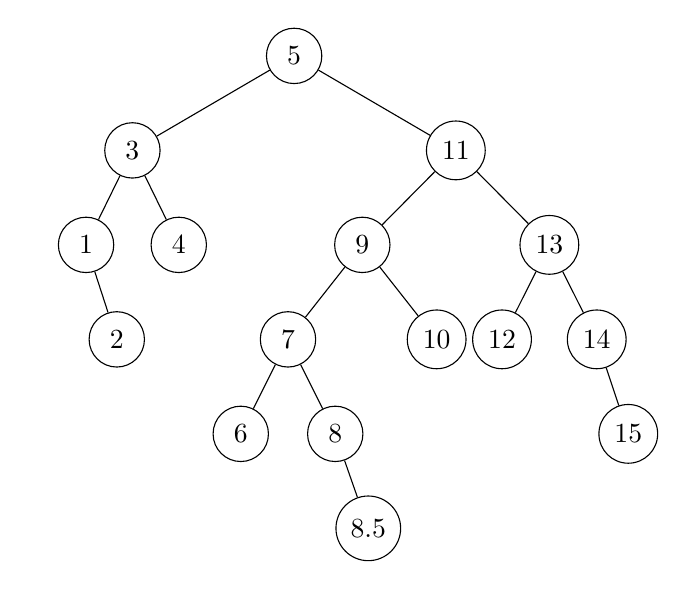
\begin{tikzpicture}[]
            \Tree
            [.5
            [.3
            [.1
            \edge[draw=none]; \node[blank]{};
            [.2
            ]
            ]
            [.4
            ]
            ]
            [.11
            [.9
            [.7
            [.6
            ]
            [.8
            \edge[blank]; \node[blank]{};
            [.8.5
            ]
            ]
            ]
            [.10
            ]
            ]
            [.13
            [.12
            ]
            [.14
            \edge[draw=none]; \node[draw=none]{};
            [.15
            ]
            ]
            ]
            ]
            ]
        \end{tikzpicture}
    \end{center}

    \part[2] Insert $8.5$ into $T$. Draw the AVL tree after balance corrections.
    \vspace{0.5cm}
    \begin{center}
        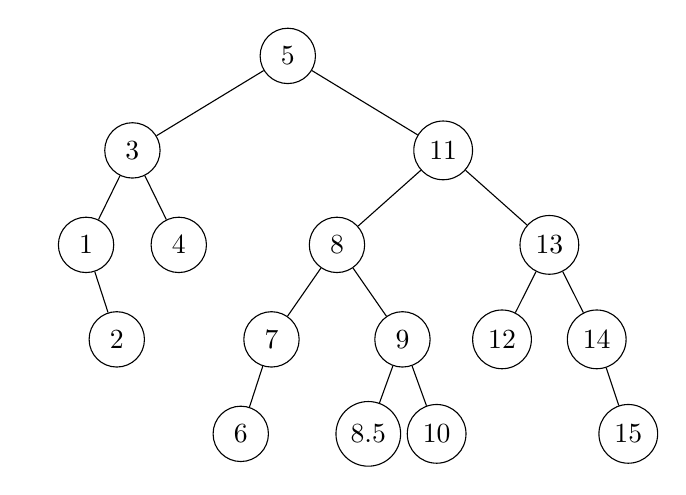
\begin{tikzpicture}[]
            \Tree
            [.5
            [.3
            [.1
            \edge[draw=none]; \node[blank]{};
            [.2
            ]
            ]
            [.4
            ]
            ]
            [.11
            [.8
                [.7
                        [.6
                        ]
                    \edge[blank]; \node[blank]{};
                ]
                [.9
                        [.8.5
                        ]
                        [.10
                        ]
                ]
            ]
            [.13
            [.12
            ]
            [.14
            \edge[draw=none]; \node[draw=none]{};
            [.15
            ]
            ]
            ]
            ]
            ]
        \end{tikzpicture}
    \end{center}

    \part[2] Remove $3$ from $T$ (\textbf{NOT from the previous answer!}). Draw the AVL tree after replacing and before checking if any balance correction is needed.
    \vspace{0.5cm}

    \begin{center}
        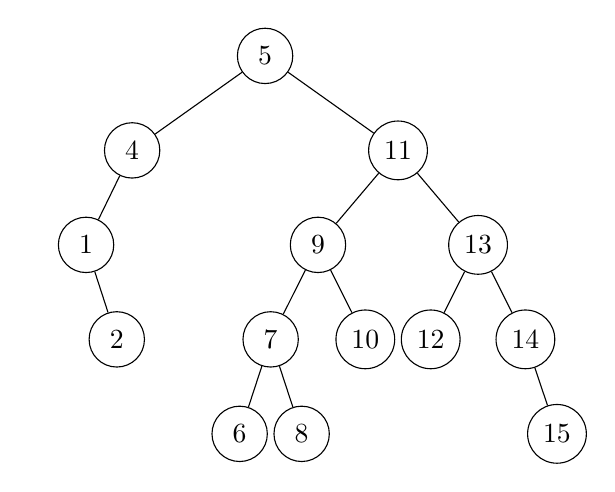
\begin{tikzpicture}[]
            \Tree
            [.5
            [.4
            [.1
            \edge[blank]; \node[blank]{};
            [.2
            ]
            ]
            \edge[blank]; \node[blank]{};
            ]
            [.11
            [.9
                [.7
                        [.6
                        ]
                        [.8
                        ]
                ]
                [.10
                ]
            ]
            [.13
            [.12
            ]
            [.14
            \edge[blank]; \node[blank]{};
            [.15
            ]
            ]
            ]
            ]
            ]
        \end{tikzpicture}
    \end{center}
    \part[2] Remove $3$ from $T$. Draw the AVL tree after balance corrections.
    \vspace{0.5cm}
    \begin{center}
        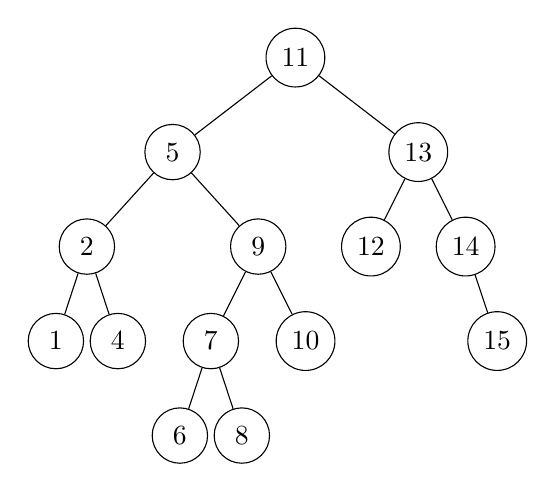
\begin{tikzpicture}[]
            \Tree
            [.11
            [.5
                [.2
                        [.1
                        ]
                        [.4
                        ]
                ]
                [.9
                        [.7
                                [.6
                                ]
                                [.8
                                ]
                        ]
                        [.10
                        ]
                ]
            ]
            [.13
            [.12
            ]
            [.14
            \edge[blank]; \node[blank]{};
            [.15
            ]
            ]
            ]
            ]
        \end{tikzpicture}
    \end{center}
\end{parts}

\end{questions}

\end{document}